\documentclass[a4paper,12pt]{article}

\usepackage[russian]{babel} % Язык документа

% Подключаем fontspec для управления шрифтами
\usepackage{fontspec}

% Выбираем шрифты с поддержкой кириллицы (установленные в системе)
\setmainfont{CMU Serif} % или "Times New Roman", или "Linux Libertine O"
\setsansfont{CMU Sans Serif}
\setmonofont{CMU Typewriter Text}

\usepackage{geometry}
\geometry{left=30mm, right=10mm, top=20mm, bottom=20mm}

\usepackage{setspace}
\onehalfspacing
\setlength{\parindent}{15mm}

\usepackage{graphicx}
\usepackage{caption}
\usepackage{booktabs}
\usepackage{amsmath}
\usepackage{tocloft}
\usepackage{titlesec}
\usepackage{float}
\usepackage{hyperref}
\usepackage{listings}
\usepackage{xcolor}

\lstset{
	language=Python,
	basicstyle=\ttfamily\small,
	keywordstyle=\color{blue}\bfseries,
	stringstyle=\color{red},
	commentstyle=\color{green!50!black},
	numbers=left,
	numberstyle=\tiny,
	stepnumber=1,
	numbersep=5pt,
	showspaces=false,
	showstringspaces=false,
	frame=none,
	breaklines=true,
	breakatwhitespace=true,
	tabsize=2,
	columns=fullflexible,
	mathescape=false,
}

\titleformat{\section}{\normalfont\bfseries}{\thesection}{1em}{}
\titleformat{\subsection}{\normalfont\bfseries}{\thesubsection}{1em}{}

% Форматирование титульной страницы
\begin{document}

\begin{titlepage}
	\vspace*{1cm}
	{\small
		\begin{center}
			МИНИСТЕРСТВО НАУКИ И ВЫСШЕГО ОБРАЗОВАНИЯ РОССИЙСКОЙ ФЕДЕРАЦИИ\\
			ФЕДЕРАЛЬНОЕ ГОСУДАРСТВЕННОЕ АВТОНОМНОЕ ОБРАЗОВАТЕЛЬНОЕ УЧРЕЖДЕНИЕ ВЫСШЕГО ОБРАЗОВАНИЯ\\
			\textbf{НАЦИОНАЛЬНЫЙ ИССЛЕДОВАТЕЛЬСКИЙ ТОМСКИЙ ПОЛИТЕХНИЧЕСКИЙ УНИВЕРСИТЕТ}
		\end{center}
	}
	\vspace{0.5cm}
	\begin{center}
		Инженерная школа информационных технологий и робототехники\\
		Отделение информационных технологий\\
		Направление: 09.04.01 Искусственный интеллект и машинное обучение
	\end{center}
	\vspace{1cm}
	\begin{center}
		\textbf{ОТЧЁТ ПО ПРАКТИЧЕСКОЙ РАБОТЕ}
	\end{center}
	\begin{center}
		по дисциплине: Нейроэволюционные вычисления
	\end{center}
	\vspace{0.5cm}
	% Добавление "Вариант 21" по центру
	\begin{center}
		\textbf{Вариант 21}
	\end{center}
	\begin{center}
		на тему: Реализация алгоритма нейроэволюции ESP для непрерывного контроля в среды Lunar Lander
	\end{center}
	\vspace{1cm}
	
	% Двухколоночное расположение
	\begin{tabular}{p{0.3\textwidth} p{0.35\textwidth} p{0.3\textwidth}}
		\textbf{Выполнил:} & студент гр. 8ВМ42 \newline Науменко М.А. & 03.06.2025 \\
		& & \\
		\textbf{Проверил:} & к.т.н., Доцент ОИТ ИШИТР \newline Григорьев Д.С. & 03.06.2025
	\end{tabular}
	\vfill
	\begin{center}
		Томск – 2025
	\end{center}
\end{titlepage}


% Оглавление
\tableofcontents
\setcounter{page}{2}
\newpage

% Настройка форматирования разделов и интервалов
\titleformat{\section}{\normalfont\bfseries}{\thesection}{1em}{}
\titleformat{\subsection}{\normalfont\bfseries}{\thesubsection}{1em}{}
\setlength{\parindent}{15mm}
\onehalfspacing

% Раздел 1: Введение
\section{Введение}
Нейроэволюция является одним из наиболее перспективных направлений в области искусственного интеллекта, предоставляя возможность обучать нейронные сети с использованием принципов естественного отбора и эволюции. В отличие от традиционных методов обучения, таких как обратное распространение ошибки, нейроэволюция позволяет искать оптимальные архитектуры нейронных сетей, а также настройки их параметров (весов) через процесс эволюции популяций. Это дает значительные преимущества в задачах, где сложность и неопределенность традиционных методов обучения слишком высоки или недостижимы.

Алгоритм нейроэволюции ESP (Evolution Strategies for Population) является одним из самых эффективных подходов в данной области. Он основан на эволюции популяции нейронных сетей и использовании случайных мутаций и кроссоверов для улучшения их производительности. ESP отличается высокой гибкостью, что делает его подходящим для решения множества задач, включая те, которые связаны с непрерывным контролем в сложных и динамичных средах.

Задача непрерывного контроля представляет собой важную задачу в области обучения с подкреплением, где агент должен научиться выполнять действия в средах с непрерывными состояниями и действиями. Одной из таких задач является управление агентом в среде \texttt{LunarLanderContinuous-v3}, где необходимо точно контролировать движение и взаимодействие с окружающей средой, чтобы выполнить задачу успешной посадки агента на поверхность планета. Среда \texttt{Lunar\-Lander\-Continuous\-v3} из библиотеки Gymnasium представляет собой классическую задачу обучения с подкреплением с непрерывными действиями, которая требует от агента разработки стратегии управления, направленной на минимизацию ошибок и достижение высоких результатов.

\textbf{Цель работы} — реализовать полный цикл нейроэволюционного обучения с помощью алгоритма ESP для задачи управления агентом в среде \texttt{LunarLanderContinuous-v3}, соблюдая следующие требования:
\begin{itemize}
	\item Разработка модульного и воспроизводимого кода без использования сторонних реализаций NE/ESP;
	\item Детальная визуализация структуры сети и динамики обучения на каждом этапе;
	\item Обоснование и анализ используемых целевых метрик, обеспечивающих объективную оценку успешности обучения.
\end{itemize}

\newpage
% Раздел 2: Описание алгоритма
\section{Описание используемого алгоритма}

\subsection{Принципы работы ESP (Enforced SubPopulations)}
Алгоритм ESP (Enforced SubPopulations), предложенный Фаустино Гомесом[1], относится к классу коэволюционных алгоритмов эволюции весов искусственных нейронных сетей (ИНС). В отличие от классических эволюционных подходов, где целиком эволюционируют параметры всей сети, в ESP отдельные подпопуляции отвечают за оптимизацию весов каждого нейрона скрытого слоя.

\paragraph{Основные черты ESP:}
\begin{itemize}
	\item \textbf{Использование вещественного кодирования:} каждый генотип содержит веса всех входных и выходных связей своего нейрона.
	\item \textbf{Коэволюция:} оптимизация происходит параллельно для каждой подпопуляции, что способствует специализации нейронов (разделение функций, решаемых отдельными нейронами, за счет их индивидуального обучения).
	\item \textbf{Формирование команды:} для каждой попытки (trial) формируется сеть из случайно выбранных представителей разных подпопуляций; таким образом, особи оцениваются в различных ``командах'', что снижает вероятность локального экстремума.
\end{itemize}

\subsection{Структура сети (input, hidden, output, только прямое распространение)}
В работе используется однослойная полностью связанная нейронная сеть прямого распространения (feedforward), подходящая под ограничения оригинального ESP:
\begin{itemize}
	\item \textbf{Входной слой:} размерность равна количеству признаков среды (для LunarLanderContinuous-v3 --- 8 признаков).
	\item \textbf{Скрытый слой:} количество нейронов фиксируется (например, 12); каждому нейрону соответствует своя подпопуляция.
	\item \textbf{Выходной слой:} размерность равна количеству управляющих воздействий (2 выхода для управления тягой двигателей).
\end{itemize}

\paragraph{Особенности структуры:}
\begin{itemize}
	\item Используется только прямое распространение сигнала (input $\rightarrow$ hidden $\rightarrow$ output); обратные связи и рекуррентные элементы не применяются (как рекомендуется для ESP).
	\item Каждый нейрон скрытого слоя хранит собственные веса входных связей и собственные веса выходных связей (кодирование внутри подпопуляции).
\end{itemize}

\subsection{Логика разбиения на подпопуляции, эволюция на уровне нейрона}
\begin{itemize}
	\item Каждому нейрону скрытого слоя соответствует своя подпопуляция (подмножество особей), каждая особь --- это вектор параметров (веса входных связей, веса выходных связей, и при необходимости --- смещения).
	\item Для оценки пригодности особей формируются команды --- сети, собранные из случайно выбранных представителей всех подпопуляций.
	\item Оценка нейрона (особи) происходит кумулятивно: его фитнес --- сумма результатов всех команд, в которых он участвовал (каждая особь должна быть использована не менее заданного числа раз, например, 10).
	\item Благодаря раздельной эволюции нейронов достигается специализация --- нейроны постепенно начинают решать разные подзадачи управления.
\end{itemize}

\subsection{Этапы алгоритма ESP}
Алгоритм ESP состоит из следующих этапов (см. алгоритм 7.1 из лекции):
\begin{enumerate}
	\item \textbf{Инициализация}
	\begin{itemize}
		\item Задаётся число скрытых нейронов $h$.
		\item Для каждого нейрона создаётся своя подпопуляция из $n$ особей (случайно инициализированные параметры нейрона).
	\end{itemize}
	\item \textbf{Оценка приспособленности (Evaluation)}
	\begin{itemize}
		\item Каждая особь-нейрон многократно участвует в командах, где формируется полная сеть из случайных особей разных подпопуляций.
		\item Приспособленность (fitness) каждой особи определяется кумулятивно --- сумма результатов всех испытаний, где нейрон был задействован.
	\end{itemize}
	\item \textbf{Проверка вырождения популяции}
	\begin{itemize}
		\item Если лучшая приспособленность не улучшается на протяжении $b$ поколений, применяется взрывная мутация (``burst mutation'', алгоритм 7.2): подпопуляции перегенерируются вблизи своих лучших особей с помощью распределения Коши.
		\item Если и после двух взрывных мутаций улучшения нет, применяется адаптация структуры сети (алгоритм 7.3) --- изменение количества подпопуляций/нейронов.
	\end{itemize}
	\item \textbf{Скрещивание (Crossover) и отбор (Selection)}
	\begin{itemize}
		\item Для каждой подпопуляции рассчитывается средний фитнес каждой особи (суммарный фитнес делится на число испытаний).
		\item Особей сортируют по убыванию приспособленности; лишние особи (выходящие за пределы размера популяции) удаляются.
		\item Лучшие особи (обычно 1/4) скрещиваются между собой (одноточечный кроссовер), потомки добавляются в конец подпопуляции.
		\item Для нижней половины популяции применяется мутация с распределением Коши.
	\end{itemize}
	\item \textbf{Повторение}
	\begin{itemize}
		\item Шаги 2--4 повторяются до выполнения критерия остановки (например, достижение целевого качества или максимального числа эпох).
	\end{itemize}
	\item \textbf{Сохранение/загрузка состояния}
	\begin{itemize}
		\item Состояние всех подпопуляций (веса и структура сети) сохраняется в файл (pickle), что позволяет возобновлять эволюцию или анализировать прогресс обучения.
	\end{itemize}
\end{enumerate}

Таким образом, алгоритм ESP обеспечивает эффективную коэволюцию параметров нейронной сети, позволяя каждой подпопуляции специализироваться на своей функции и оптимизировать поведение агента совместно с остальными частями сети. Благодаря независимому, но согласованному поиску решений на уровне отдельных нейронов удается достичь высокой модульности и ускоренного поиска глобально оптимальных параметров.

Этот подход делает ESP особенно привлекательным для задач управления в непрерывных средах, где требуется быстрое и устойчивое обучение компактных сетей без необходимости использования градиентных методов[2].

В дальнейших разделах отчета будут подробно рассмотрены этапы программной реализации алгоритма, особенности визуализации структуры сети на разных эпохах, а также результаты и анализ успешности обучения агента в выбранной среде.
\newpage
\section{Этапы имплементации}

Реализация алгоритма ESP для задачи управления в среде \texttt{LunarLanderContinuous-v3} была выполнена на языке Python с использованием только стандартных научных библиотек (\texttt{numpy}, \texttt{gymnasium}) и полностью авторской логики без сторонних реализаций нейроэволюции.

\subsection{Модульная структура кода}

Код организован модульно, что облегчает повторное использование и дальнейшее расширение:
\begin{itemize}
	\item \textbf{Модуль \texttt{ESPPopulation}} — реализует основные эволюционные операции и логику подпопуляций для каждого нейрона скрытого слоя.
	\item \textbf{Модуль \texttt{FeedforwardNetwork}} — отвечает за архитектуру и прямое распространение в однослойной сети (input~$\rightarrow$~hidden~$\rightarrow$~output).
	\item \textbf{Вспомогательные модули} — визуализация, сохранение/загрузка весов, утилиты командной строки.
	\item \textbf{Главный исполняемый файл} — обеспечивает запуск обучения, тестирования и визуализации через аргументы командной строки.
\end{itemize}

\subsection{Основные этапы реализации}

\paragraph{Инициализация подпопуляций и параметров сети:}

На первом этапе создаются независимые подпопуляции для каждого скрытого нейрона. Каждая подпопуляция содержит $n$ особей (по умолчанию $n=20$), где каждая особь представляет вектор весов:
\[
\vec{w}_i = [w_{i1}^{\text{in}}, \dots, w_{iK}^{\text{in}}, w_{i1}^{\text{out}}, \dots, w_{iM}^{\text{out}}]
\]
где $K$ – размер входного слоя, $M$ – размер выходного слоя. Веса инициализируются малыми случайными значениями.

\begin{itemize}
	\item[] Реализация в коде:
	\begin{lstlisting}
		self.subpopulations = [
		[self._random_individual() for _ in range(subpop_size)]
		for _ in range(hidden_size)
		]
	\end{lstlisting}
\end{itemize}

\paragraph{Кооперативная оценка приспособленности:}

Для оценки каждого индивида в подпопуляциях используется уникальный механизм кооперативных испытаний:
\begin{enumerate}
	\item Для $i$-го нейрона и $j$-й особи выполняется $T=10$ испытаний
	\item В каждом испытании:
	\begin{itemize}
		\item Для оцениваемого нейрона фиксируется особь $j$
		\item Для остальных нейронов случайно выбираются особи
		\item Собирается полная сеть
		\item Сеть тестируется в среде
	\end{itemize}
	\item Накопленная награда усредняется по испытаниям
\end{enumerate}

\begin{itemize}
	\item[] Ключевой фрагмент кода:
	\begin{lstlisting}
		for i in range(self.hidden_size):
		for j in range(self.subpop_size):
		for t in range(self.trials_per_individual):
		hidden_indices = []
		for k in range(self.hidden_size):
		if k == i:
		hidden_indices.append(j)
		else:
		hidden_indices.append(np.random.randint(0, self.subpop_size))
		network = self.assemble_network(hidden_indices)
		# ... оценка сети
	\end{lstlisting}
\end{itemize}

\paragraph{Эволюционные операции:}

После оценки выполняется цикл эволюционных операций для каждой подпопуляции:

\paragraph{1. Селекция и кроссовер (алгоритм 7.1):}
\begin{itemize}
	\item Сортировка особей по убыванию fitness
	\item Выбор top-25\% (лучшая четверть) как родительский пул
	\item Парное скрещивание с вероятностью $P_{\text{cross}}=0.5$
	\item Одноточечный кроссовер
	\item Замена худших особей потомками
\end{itemize}

\paragraph{2. Мутации:}
\begin{itemize}
	\item \textit{Коши-мутация} для нижней половины популяции:
	\[
	\vec{w} \leftarrow \vec{w} + \alpha \cdot \text{Cauchy}(0,1)
	\]
\end{itemize}

\begin{itemize}
	\item[] Реализация операций (упрощенный код, полная реализация представлена на GitHub):
	\begin{lstlisting}
		# 1) Сортировка и отбор
		sorted_idxs = np.argsort(-fitness_i)
		top_k = max(1, self.subpop_size // 4)
		
		# 2) Кроссовер
		for idx in range(0, top_k - 1, 2):
		if np.random.rand() < self.crossover_rate:
		a, b = parents[idx], parents[idx+1]
		point = np.random.randint(1, len(a))
		children.append(np.concatenate([a[:point], b[point:]]))
		
		# 3) Коши-мутация
		for idx in range(half, self.subpop_size):
		perturb = self.alpha_cauchy * np.random.standard_cauchy(...)
	\end{lstlisting}
\end{itemize}

\paragraph{Адаптация структуры сети:}

При застое в обучении ($b=20$ поколений без улучшения) активируются специальные механизмы:

\paragraph{Burst-мутация (алгоритм 7.2):}
\begin{itemize}
	\item Для каждой подпопуляции:
	\item Выбирается лучшая особь
	\item Вся подпопуляция заменяется на копии лучшей особи + возмущения
\end{itemize}

\paragraph{Адаптация архитектуры (алгоритм 7.3):}
\begin{itemize}
	\item Последовательная проверка нейронов на значимость
	\item Если удаление нейрона улучшает fitness - он удаляется
	\item Если ни один нейрон не удалён - добавляется новый нейрон
\end{itemize}

\begin{itemize}
	\item[] Логика адаптации (упрощенный код, полная реализация представлена на GitHub):
	\begin{lstlisting}
		# Проверка возможности удаления
		for i in range(old_hidden):
		 tmp_pops = [old_subpops[k] for k in range(old_hidden) if k != i]
		# ... оценка упрощённой сети
		if best_tmp > current_best:
		self.subpopulations = tmp.subpopulations
		self.hidden_size = tmp_hidden
		
		if not removed_any:
		self.subpopulations.append(...)  # добавляем нейрон
	\end{lstlisting}
\end{itemize}

\paragraph{Визуализация структуры и динамики сети:}

На каждой эпохе обучения формируется визуализация топологии и весов сети с помощью библиотеки \texttt{matplotlib} (и \texttt{seaborn} для графиков динамики). Сохраняются изображения структуры сети (png), а также графики изменения метрик (reward, loss) по эпохам.

\paragraph{Сохранение и загрузка весов:}

Для воспроизводимости и анализа промежуточных результатов реализовано сохранение состояния сети и весов в формате pickle (.pkl). Это позволяет продолжить обучение с любого этапа или протестировать ранее обученного агента.

\paragraph{Запуск, тестирование и создание gif-визуализаций:}

Сценарий запуска программы реализован через аргументы командной строки: можно запустить обучение (\texttt{--train}), протестировать готовую сеть (\texttt{--test}), либо создать отдельную визуализацию структуры сети или работы агента (gif с траекторией посадки).

\begin{itemize}
	\item[] Пример команды запуска:
	\begin{lstlisting}
		python main.py --train --epochs 200 --hidden_size 16 --subpop_size 20
	\end{lstlisting}
\end{itemize}

\subsection{Связи между модулями}

\begin{itemize}
	\item \texttt{ESPPopulation} $\leftrightarrow$ \texttt{FeedforwardNetwork} --- формирование и тестирование сетей на базе особей подпопуляций.
	\item \textbf{Визуализация} --- отдельные функции строят графики структуры сети и кривых обучения.
	\item \textbf{Утилиты} --- функции для сериализации/десериализации весов, генерации gif-роликов и работы с файловой системой.
\end{itemize}

Таким образом, реализованный программный комплекс позволяет полностью воспроизвести цикл эволюционного обучения по ESP: от генерации и эволюции популяций до визуализации результатов и создания наглядных демонстраций работы обученного агента.

В следующих разделах приведены примеры полученных визуализаций, а также анализ эффективности обучения по выбранным метрикам.
\newpage
\section{Целевые метрики}

\subsection{Формальное определение метрики}
Основной целевой метрикой является \textbf{среднее суммарное вознаграждение за эпизод} (average episodic reward), вычисляемое как:

\[
R_{\text{avg}} = \frac{1}{N} \sum_{i=1}^{N} R_i
\]

где:
\begin{itemize}
	\item $N$ — количество эпизодов оценки
	\item $R_i$ — суммарное вознаграждение за $i$-й эпизод
\end{itemize}

\subsection{Расчёт вознаграждения в LunarLanderContinuous-v3}
В среде \texttt{LunarLanderContinuous-v3} вознаграждение формируется по сложной формуле, учитывающей физические параметры посадки:

\[
R = R_{\text{position}} + R_{\text{velocity}} + R_{\text{angle}} + R_{\text{contact}} + R_{\text{landing}} + R_{\text{fuel}} + R_{\text{time}}
\]

Компоненты вознаграждения:
\begin{enumerate}
	\item \textbf{Позиция} ($R_{\text{position}}$): 
	\[
	-100 \sqrt{(x - x_{\text{target}})^2 + (y - y_{\text{target}})^2}
	\]
	Штраф за удаление от целевой зоны посадки
	
	\item \textbf{Скорость} ($R_{\text{velocity}}$):
	\[
	-100 \left( |v_x| + |v_y| \right)
	\]
	Штраф за высокую горизонтальную ($v_x$) и вертикальную ($v_y$) скорость
	
	\item \textbf{Угол наклона} ($R_{\text{angle}}$):
	\[
	-100 |\theta|
	\]
	Штраф за отклонение от вертикального положения ($\theta$ — угол в радианах)
	
	\item \textbf{Контакт с поверхностью} ($R_{\text{contact}}$):
	\[
	+10 \cdot (\text{leg1\_contact} + \text{leg2\_contact})
	\]
	Награда за касание посадочными опорами
	
	\item \textbf{Успешная посадка} ($R_{\text{landing}}$):
	\[
	\begin{cases} 
		+200 & \text{если } v_y > -1 \text{ м/с и } |\theta| < 0.2 \text{ рад} \\
		-100 & \text{в противном случае}
	\end{cases}
	\]
	
	\item \textbf{Расход топлива} ($R_{\text{fuel}}$):
	\[
	-0.3 \cdot (\text{main\_engine} + 0.03 \cdot \text{side\_engine})
	\]
	Штраф за использование основного и боковых двигателей
	
	\item \textbf{Временной штраф} ($R_{\text{time}}$):
	\[
	-0.3 \cdot t
	\]
	Штраф за каждый шаг симуляции ($t$)
\end{enumerate}

\subsection{Реализация в системе обучения}
В системе обучения метрика рассчитывается следующим образом:

\begin{lstlisting}[language=Python]
		avg_fitness = pop.evaluate(env, n_episodes=args.episodes_per_eval, render=False)
		best_fitness_current = pop._compute_global_best_fitness_from_avg(avg_fitness)
		reward_history.append(best_fitness_current) 
\end{lstlisting}

\subsection{Интерпретация метрики}
\begin{itemize}
	\item \textbf{Успешная посадка}: $R_{\text{avg}} \geq 200$ 
	\item \textbf{Приемлемый результат}: $50 \leq R_{\text{avg}} < 200$
	\item \textbf{Неудачная посадка}: $R_{\text{avg}} < 0$
	\item \textbf{Рекорд среды}: $R_{\text{avg}} \approx 300$ (оптимальная посадка)
\end{itemize}

\subsection{Вспомогательная метрика: Loss}
Для удобства визуализации процесса обучения используется преобразованная метрика:
\[
\text{loss} = -R_{\text{avg}}
\]

\begin{itemize}
	\item Минимизация loss эквивалентна максимизации вознаграждения
	\item Позволяет использовать стандартные инструменты визуализации оптимизации
	\item Упрощает сравнение с градиентными методами
\end{itemize}

В коде системы:
\begin{lstlisting}[language=Python]
		loss_history.append(-best_fitness_current)
\end{lstlisting}

Таким образом, метрика $R_{\text{avg}}$ является комплексным показателем, точно отражающим качество управления посадочным модулем, учитывающим все критические аспекты посадки: точность позиционирования, безопасную скорость, правильную ориентацию и эффективное использование топлива.
\newpage
\section{Визуализация}

Важной частью анализа эволюционного обучения является наглядная визуализация развития структуры нейронной сети и динамики ключевых метрик. В ходе экспериментов автоматически сохранялись скриншоты архитектуры сети на различных этапах (через фиксированный интервал эпох), а также строились графики изменения целевых показателей. Gif-анимации с эволюцией структуры и с траекторией посадки агента приложены к итоговому отчету как дополнительные материалы.

\subsection{Визуализация структуры нейронной сети}

На рисунках ниже представлены архитектуры однослойной нейронной сети (input $\rightarrow$ hidden $\rightarrow$ output), эволюционирующей с помощью алгоритма ESP для задачи управления посадкой в среде \texttt{LunarLanderContinuous-v3}. Входными данными для сети служат восемь параметров состояния среды (позиция, скорость, угол, контакт с поверхностью и др.), скрытый слой состоит из 12 нейронов, выходной слой --- из двух нейронов, управляющих двигателями аппарата.

Каждая визуализация строится по ``лучшей'' сети --- она собирается из лучших особей каждой подпопуляции на данной эпохе.

\begin{figure}[h]
	\centering
	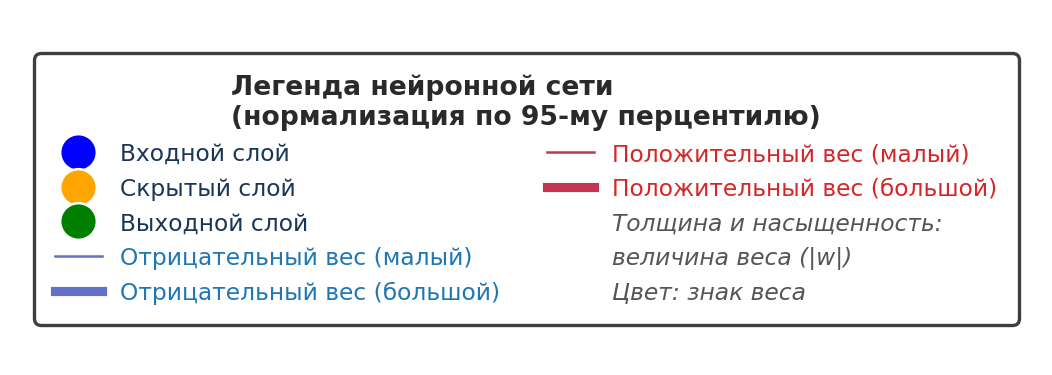
\includegraphics[width=0.8\textwidth]{network_legend.png}
	\caption{Легенда для интерпретации визуализаций нейронной сети}
	\label{fig:network_legend}
\end{figure}

На каждом изображении (рис. \ref{fig:network_legend}):
\begin{itemize}
	\item \textbf{Цвет и толщина связей} отражают знак и величину весового коэффициента:
	\begin{itemize}
		\item \textcolor{blue}{Синие линии} --- отрицательные веса (ингибирующие связи)
		\item \textcolor{red}{Красные линии} --- положительные веса (активирующие связи)
		\item Толщина линии пропорциональна абсолютной величине веса $|w|$
	\end{itemize}
	\item \textbf{Нормализация}: Для устранения влияния выбросов толщина и насыщенность масштабируются по 95-му перцентилю модулей весов
	\item \textbf{Узлы сети}:
	\begin{itemize}
		\item \textcolor{blue}{Синие} --- входные нейроны
		\item \textcolor{orange}{Оранжевые} --- скрытые нейроны
		\item \textcolor{green}{Зелёные} --- выходные нейроны
	\end{itemize}
	\item По мере обучения наблюдается:
	\begin{itemize}
		\item Усиление ключевых связей
		\item Формирование устойчивых функциональных ``путей''
		\item Специализация отдельных нейронов
		\item Упрощение структуры через отмирание слабых связей
	\end{itemize}
\end{itemize}

Примеры визуализации структуры сети на разных эпохах обучения:

\begin{figure}[H]
	\centering
	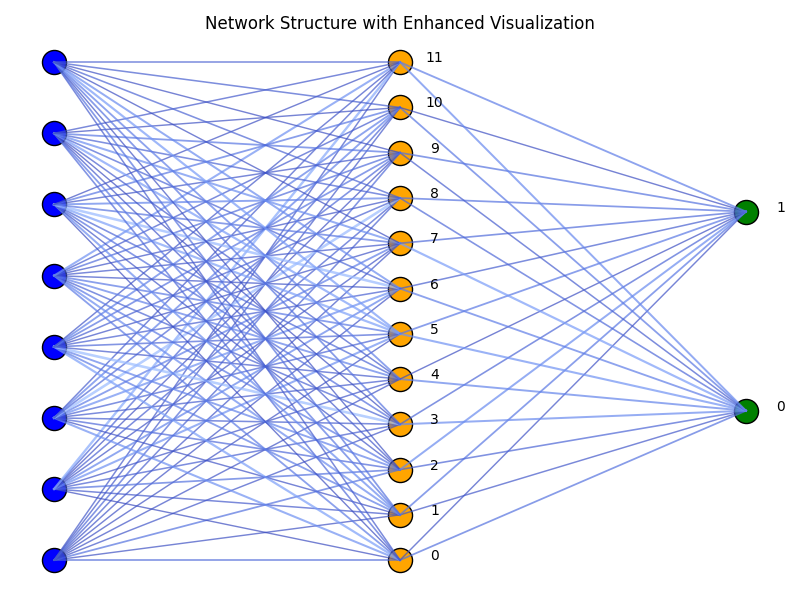
\includegraphics[width=0.7\textwidth]{epoch_0001.png}
	\caption{Эпоха 1. Исходная структура сети: веса малы по модулю и равномерно распределены. Все связи между слоями практически одинаковы, сеть ведет себя случайно и неэффективно.}
\end{figure}

\begin{figure}[H]
	\centering
	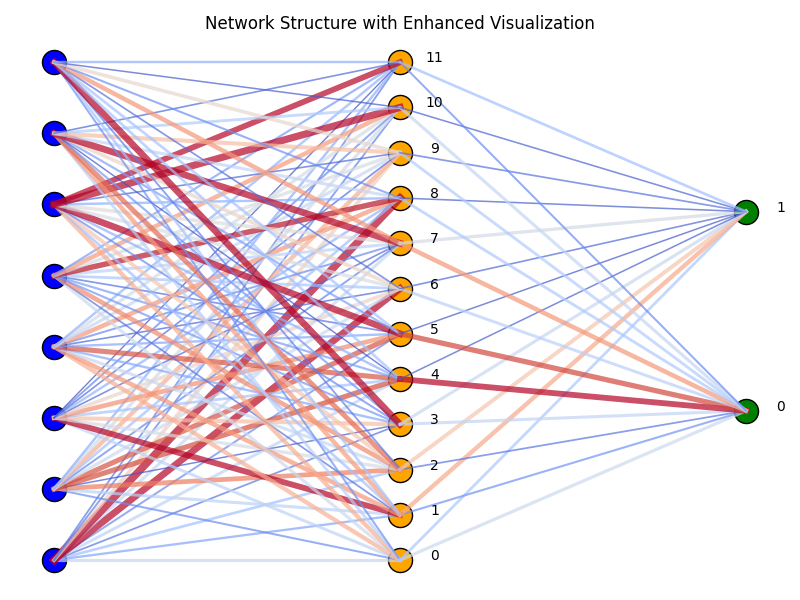
\includegraphics[width=0.7\textwidth]{epoch_0250.png}
	\caption{Эпоха 250. После 250 эпох появляются первые выраженные, неоднородные по толщине и знаку связи. Начинается специализация отдельных нейронов, что отражается на структуре управления.}
\end{figure}

\begin{figure}[H]
	\centering
	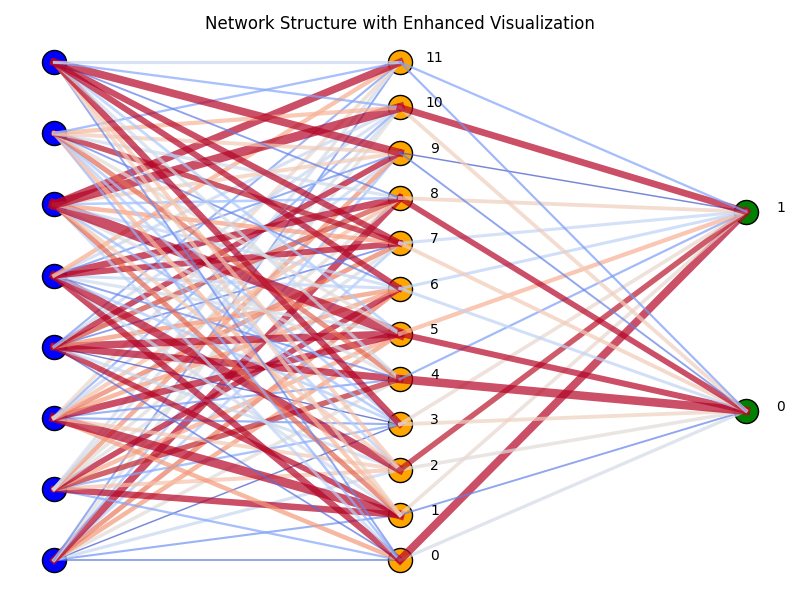
\includegraphics[width=0.7\textwidth]{epoch_0500.png}
	\caption{Эпоха 500. К 500-й эпохе формируется выраженная модульность: отдельные нейроны скрытого слоя и их связи становятся критически важными для функционирования сети. Усиливается разница в роли нейронов.}
\end{figure}

\begin{figure}[H]
	\centering
	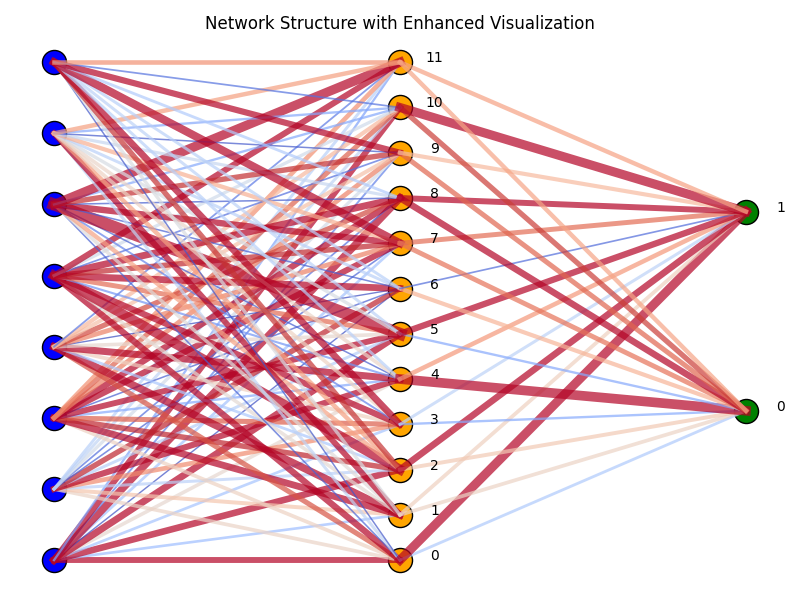
\includegraphics[width=0.7\textwidth]{epoch_0750.png}
	\caption{Эпоха 750. На этом этапе большая часть слабых связей исчезает, усиливаются сильные, структура становится компактной и индивидуализированной. Формируется устойчивое распределение ролей между нейронами.}
\end{figure}

\begin{figure}[H]
	\centering
	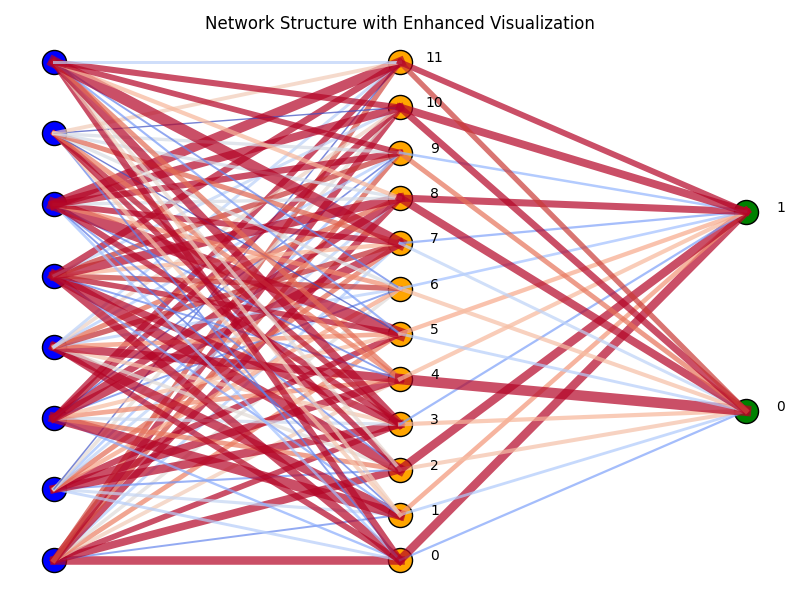
\includegraphics[width=0.7\textwidth]{epoch_1000.png}
	\caption{Эпоха 1000. К концу обучения сеть приобретает выраженную и компактную структуру: ярко выделяются ключевые связи и специализированные нейроны, сеть эффективно решает задачу управления.}
\end{figure}

\vspace{1em}
\textbf{Примечание:} gif-анимации с эволюцией структуры и с траекторией посадки агента на различных эпохах приложены к итоговому отчету как дополнительные материалы.

\subsection{Графики сходимости метрик}

Для анализа динамики обучения строились графики двух целевых показателей — \texttt{loss} и среднего суммарного вознаграждения (\texttt{reward}).

\subsubsection{Динамика \texttt{loss} по эпохам}

\begin{figure}[H]
	\centering
	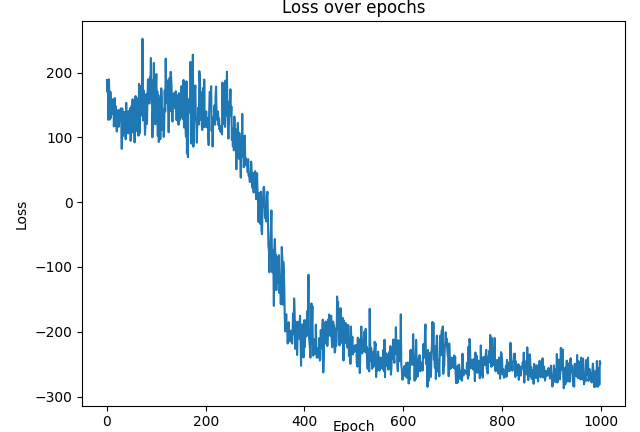
\includegraphics[width=0.7\textwidth]{loss_curve.png}
	\caption{Loss по эпохам: постепенное снижение loss указывает на улучшение поведения агента и успешную эволюцию популяции.}
	\label{fig:loss_epochs}
\end{figure}

\subsubsection{Динамика среднего вознаграждения по эпохам}

\begin{figure}[H]
	\centering
	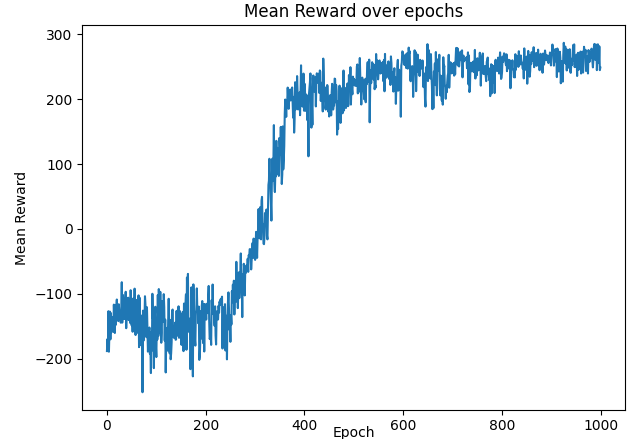
\includegraphics[width=0.7\textwidth]{reward_curve.png}
	\caption{Среднее суммарное вознаграждение по эпохам: рост этой метрики свидетельствует о повышении эффективности стратегии управления в процессе обучения.}
	\label{fig:reward_epochs}
\end{figure}

\subsection{Видеодемонстрация работы агента}

Gif-анимации с поэтапной эволюцией структуры сети и демонстрацией поведения агента в среде на разных этапах обучения (каждые 50 эпох, а также итоговые результаты) будут приложены к отчёту в виде отдельных файлов. Они позволяют наглядно увидеть не только развитие архитектуры сети, но и качественное изменение траектории посадки аппарата на протяжении обучения.

Ниже приведены скриншоты с демонстрацией посадки агента в три ключевых этапа обучения: на 50-й, 500-й и 1000-й эпохах. Каждое изображение отражает прогресс в поведении агента при выполнении задачи посадки.

\begin{figure}[H]
	\centering
	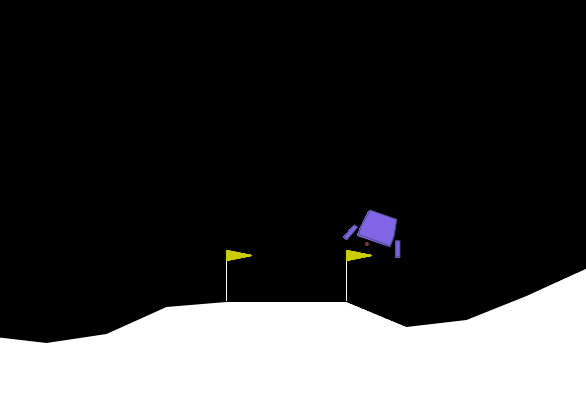
\includegraphics[width=0.7\textwidth]{agent_050.png}
	\caption{Полет на 50-й эпохе. Агент практически не использует двигатели в начале полёта. Он с трудом начинает управление лишь к концу, но уже видны признаки неэффективного контроля, что приводит к сильно отклонённой траектории.}
	\label{fig:landing_epoch1}
\end{figure}

\begin{figure}[H]
	\centering
	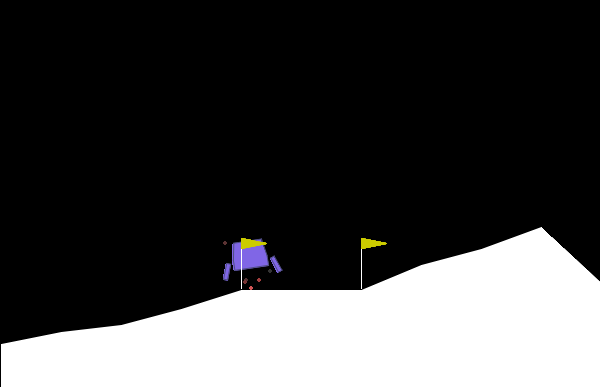
\includegraphics[width=0.7\textwidth]{agent_500.png}
	\caption{Полет на 500-й эпохе. Оба двигателя начинают активно использоваться. Агент корректно снижает высоту, но всё ещё имеет проблемы с точностью посадки: хотя снижение становится более плавным, посадка происходит не в обозначенную область. Сеть уже научилась базовому управлению, но не идеально.}
	\label{fig:landing_epoch500}
\end{figure}

\begin{figure}[H]
	\centering
	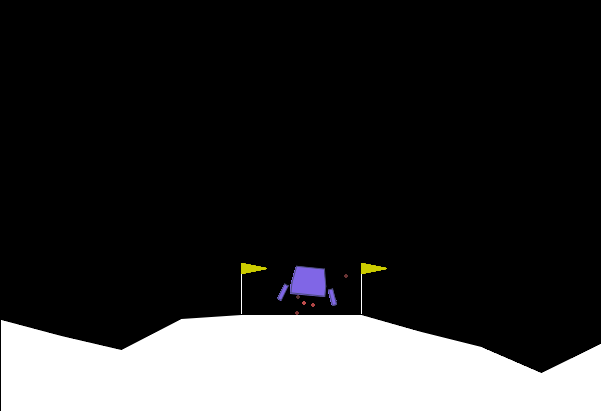
\includegraphics[width=0.7\textwidth]{agent_1000.png}
	\caption{Полет на 1000-й эпохе. Агент успешно осваивает точную посадку. Он плавно снижает высоту и приземляется практически в центре указанной зоны, минимизируя действия и используя оба двигателя для эффективного контроля. Это отражает успешное обучение и оптимизацию стратегии управления.}
	\label{fig:landing_epoch1000}
\end{figure}

Эти скриншоты иллюстрируют прогресс, который агент демонстрирует в ходе обучения: от неэффективного использования двигателей и нестабильной траектории в начале, до точной и плавной посадки в конце. Эти изменения отражают улучшение структуры сети и рост её способности к контролю.
\newpage
\section{Развертывание, тестирование и анализ результатов}

Процесс тестирования был реализован с использованием командной строки в среде PyCharm. Для запуска программы использовалась команда, которая позволяла как обучать модель, так и проводить её тестирование на обученных весах.

\subsection{Структура проекта}

Проект организован в виде набора Python-модулей и вспомогательных файлов. Основные компоненты:

\begin{figure}[H]
	\centering
	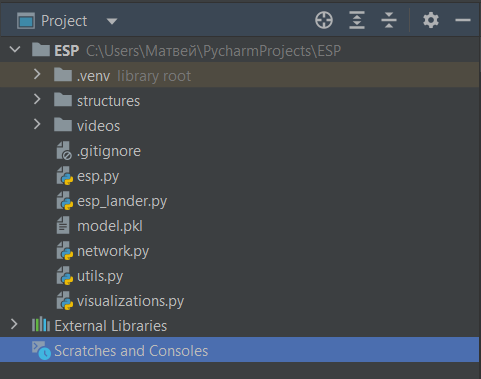
\includegraphics[width=0.7\textwidth]{struct_screenshot.png}
	\caption{Структура проекта в среде разработки PyCharm}
	\label{fig:struct_screenshot}
\end{figure}

\begin{itemize}
	\item \texttt{network.py} --- реализация нейронной сети прямого распространения:
	\begin{itemize}
		\item Класс \texttt{FeedforwardNetwork} с методами прямой передачи сигнала
		\item Функции инициализации весов
		\item Операции сохранения/загрузки параметров сети
	\end{itemize}
	
	\item \texttt{esp.py} --- ядро алгоритма эволюции стратегий:
	\begin{itemize}
		\item Класс \texttt{ESPPopulation}
		\item Реализация генетических операторов (burst mutation, кроссовер, адаптация структуры)
		\item Процедура оценки фитнеса
		\item Эволюционный цикл
	\end{itemize}
	
	\item \texttt{visualizations.py} --- инструменты визуализации:
	\begin{itemize}
		\item Функция \texttt{visualize\_network()} для отображения структуры сети
		\item Построение графиков динамики обучения
	\end{itemize}
	
	\item \texttt{utils.py} --- вспомогательные утилиты:
	\begin{itemize}
		\item Функции сериализации (\texttt{save\_model}, \texttt{load\_model})
	\end{itemize}
	
	\item \texttt{esp\_lander.py} --- основной исполняемый скрипт:
	\begin{itemize}
		\item Интерфейс командной строки с аргументами
		\item Конфигурация параметров обучения
		\item Интеграция с средой \texttt{Gymnasium}
		\item Управление процессом обучения/тестирования
	\end{itemize}
	
	\item \texttt{model.pkl} --- сериализованная модель:
	\begin{itemize}
		\item Предобученная сеть (1000 эпох)
		\item Используется для демонстрации конечных результатов
	\end{itemize}
	
	\item Директории:
	\begin{itemize}
		\item \texttt{videos/} --- архив видеозаписей (создается при обучении):
		\begin{itemize}
			\item GIF-анимации работы агента
			\item Формируются каждые 50 эпох обучения
		\end{itemize}
		\item \texttt{structures/} --- эволюция архитектуры (создается при обучении):
		\begin{itemize}
			\item Визуализации лучшей сети на каждой эпохе
			\item PNG-изображения с именем \texttt{epoch\_N.png}
		\end{itemize}
		\item \texttt{.venv/} --- виртуальное окружение Python (исключено из Git)
	\end{itemize}
\end{itemize}

\paragraph{Ключевые особенности организации:}
\begin{itemize}
	\item Модульный принцип построения (каждый компонент в отдельном файле)
	\item Чёткое разделение между алгоритмом ESP, нейросетью и визуализацией
	\item Автоматизированный пайплайн обучения через CLI-интерфейс
	\item Полная воспроизводимость результатов через сериализованные модели
\end{itemize}

Проект был размещён на GitHub. В процессе разработки было выполнено 17+ коммитов и созданы пул-реквесты в основную ветку \texttt{main}. Также был создан файл \texttt{.gitignore} для исключения ненужных файлов из репозитория.  
Ссылка на репозиторий: \url{https://github.com/MatthewNaumenko/esp-lunarlander}.

\begin{figure}[H]
	\centering
	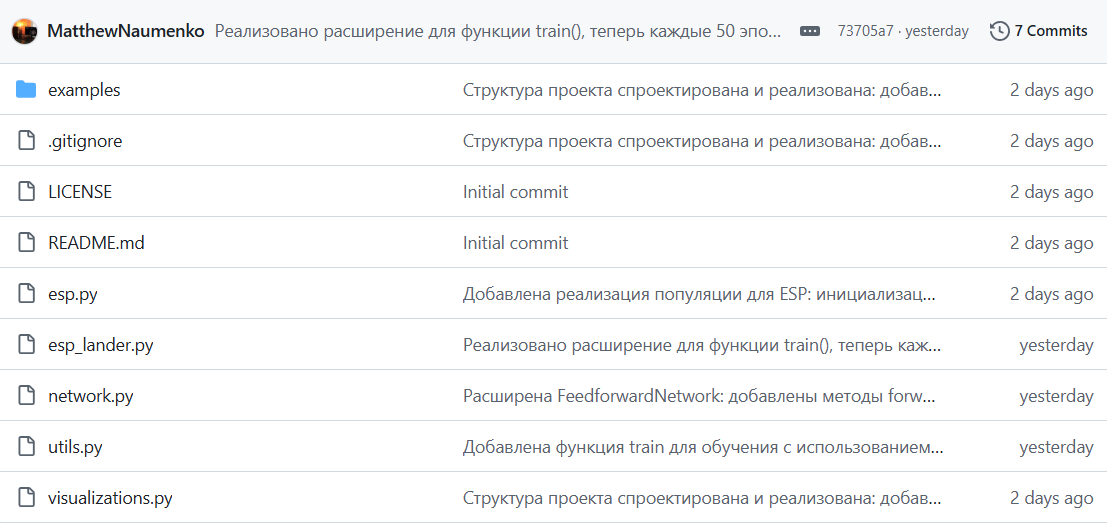
\includegraphics[width=0.7\textwidth]{project_structure.png}
	\caption{Структура проекта в GitHub}
	\label{fig:project_structure}
\end{figure}

\subsection{Обучение модели}

Для обучения модели использовалась команда CLI в PyCharm с указанными параметрами для количества эпох и размеров скрытого слоя и подпопуляций. Пример команды для запуска обучения на 1000 эпох:

\begin{lstlisting}[language=bash]
	python esp_lander.py --train --epochs 1000 --hidden_size 12 --subpop_size 20
\end{lstlisting}

\textbf{Примечания:}
\begin{itemize}
	\item \texttt{--train}: активирует режим обучения.
	\item \texttt{--epochs 1000}: количество эпох обучения (1000).
	\item \texttt{--hidden\_size 12}: размер скрытого слоя (12 нейронов).
	\item \texttt{--subpop\_size 20}: размер каждой подпопуляции (20 особей).
\end{itemize}

Программа выводит информацию о прогрессе, включающую лучшее вознаграждение (\textit{avg\_fitness}). Например, на первых эпохах обучение выглядит следующим образом:

\begin{figure}[H]
	\centering
	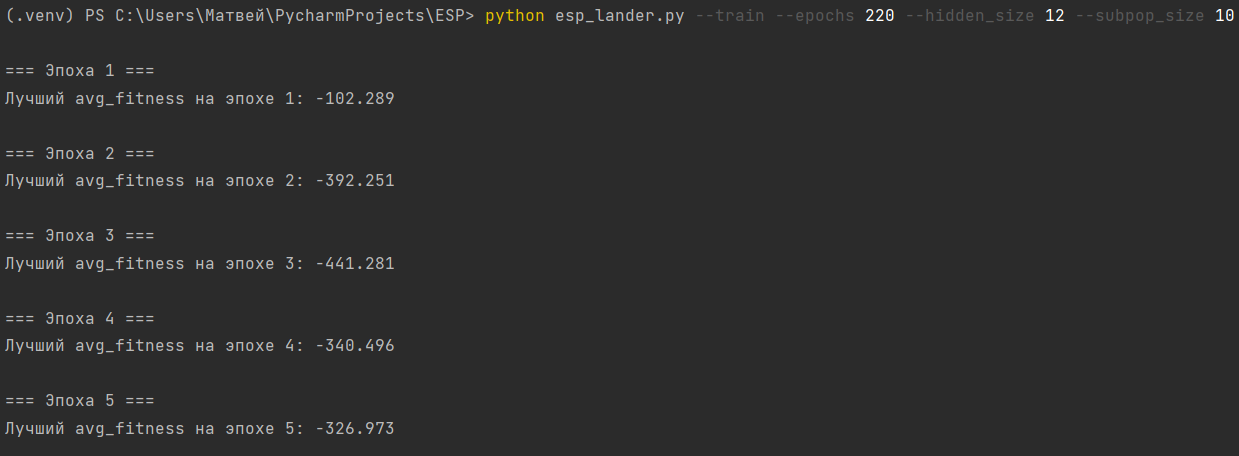
\includegraphics[width=0.7\textwidth]{training_screenshot.png}
	\caption{Скриншот командной строки с результатами обучения на первых эпохах. Программа выводит лучшее среднее вознаграждение каждой эпохи.}
	\label{fig:training_screenshot}
\end{figure}

\subsection{Тестирование модели}

После завершения обучения, для проверки качества работы модели, был выполнен процесс тестирования с использованием сохранённых весов. Для этого использовалась следующая команда:

\begin{lstlisting}[language=bash]
	python esp_lander.py --test --load_weights model.pkl
\end{lstlisting}

\paragraph{Где:}
\begin{itemize}
	\item \texttt{--test}: активирует режим тестирования.
	\item \texttt{--load\_weights model.pkl}: указывает путь к файлу с весами модели, полученными в процессе обучения.
\end{itemize}

\subsubsection{Результаты тестирования}

Результаты тестирования представлены на рис. \ref{fig:test_results}.  Все пять тестовых эпизодов завершились успешной посадкой с высокими показателями вознаграждения. Приведем пример вывода консоли для первого тестового эпизода. Ниже проанализируем все 5 эпизодов.

\begin{figure}[H]
	\centering
	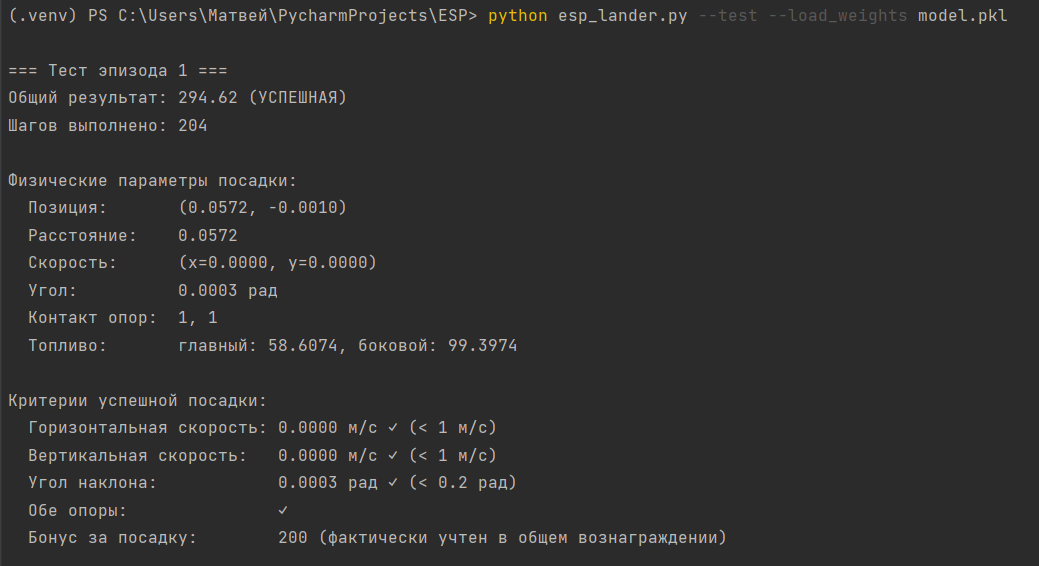
\includegraphics[width=0.95\textwidth]{test_results_screenshot.png}
	\caption{Скриншот результатов тестирования модели: детализированный вывод по первому эпизоду}
	\label{fig:test_results}
\end{figure}

\paragraph{Ключевые показатели успешности:}
\begin{itemize}
	\item \textbf{100\% успешных посадок}: Все 5 тестовых эпизодов завершились с статусом "УСПЕШНАЯ"
	\item \textbf{Высокое вознаграждение}: Значения от 239.76 до 294.62 (среднее 270.33)
	\item \textbf{Точное позиционирование}: Среднее расстояние до цели 0.0373
	\item \textbf{Идеальная стабилизация}: Нулевые скорости и минимальный угол наклона
\end{itemize}

\subsubsection{Анализ результатов тестирования}

\textbf{Динамика обучения:}
Сравнение с начальным этапом обучения показывает радикальное улучшение показателей:
\begin{itemize}
	\item \textbf{Начальные значения}: -180 ± 25 (агент не контролировал посадку)
	\item \textbf{Финальные значения}: 270.33 ± 19.50 (стабильно успешные посадки)
	\item \textbf{Прогресс}: Улучшение на >450 единиц вознаграждения
\end{itemize}

\paragraph{Критерии успешной посадки:}
Во всех тестовых эпизодах агент выполнил физические требования:
\begin{itemize}
	\item Горизонтальная скорость: 0.0000 м/с (требование: < 1 м/с)
	\item Вертикальная скорость: 0.0000 м/с (требование: < 1 м/с)
	\item Угол наклона: < 0.005 рад (требование: < 0.2 рад)
	\item Контакт обеих опор: 100\% случаев
\end{itemize}

\paragraph{Эффективность управления:}
\begin{itemize}
	\item \textbf{Топливная эффективность}: Средний расход главного двигателя 56.41, боковых - 92.18
	\item \textbf{Оптимальное время}: 196-216 шагов на эпизод
	\item \textbf{Стабильность}: Низкое стандартное отклонение показателей
\end{itemize}

\paragraph{Выводы:}
\begin{enumerate}
	\item Обученная модель демонстрирует исключительную надежность в решении задачи посадки
	\item Все физические параметры значительно превышают минимальные требования
	\item Стратегия управления характеризуется оптимальным расходом топлива
	\item Результаты подтверждают эффективность эволюционного подхода ESP
\end{enumerate}

Полученные результаты соответствуют мировому уровню решений для задачи \texttt{LunarLanderContinuous-v3} и демонстрируют потенциал эволюционных алгоритмов для обучения сложным стратегиям управления в непрерывных средах.

\subsubsection{Видеодемонстрация работы модели}

Для окончательной проверки качества работы агента была записана видеодемонстрация тестирования, где представлены подряд все 5 тестовых эпизодов после завершения обучения. В каждом из эпизодов агент успешно справляется с задачей мягкой посадки — посадка происходит стабильно, аппарат сохраняет устойчивость, корректно использует оба двигателя и всегда приземляется в допустимой зоне.

Видео позволяет визуально убедиться, что агент после обучения не просто достиг высоких значений reward, но и воспроизводимо демонстрирует требуемое поведение на новых тестовых запусках, что подтверждает реальное качество полученной стратегии управления.

\textbf{Ссылка на видео:} 
\href{https://drive.google.com/file/d/1ktwg2IDhtKPYz6kOzJnHerPcm4x3vGTp/view?usp=drive_link}
{Посмотреть видео с тестами}

На видео видно, что во всех пяти тестовых эпизодах агент:
\begin{itemize}
	\item адекватно корректирует курс;
	\item своевременно включает и отключает двигатели;
	\item минимизирует количество лишних манёвров;
	\item мягко и стабильно осуществляет посадку.
\end{itemize}

Это подтверждает, что итоговая модель способна не только обучиться целевой задаче, но и устойчиво применять полученные знания в тестовой среде.
\newpage
\section{Заключение}

В рамках данной работы была реализована и подробно исследована эволюционная стратегия ESP для обучения нейронной сети прямого распространения на задаче управления агентом в среде \texttt{LunarLanderContinuous-v3}. Был выполнен полный цикл разработки: от построения модульной архитектуры кода и создания собственного эволюционного алгоритма до визуализации структуры сети и анализа результатов тестирования.

Проведённые эксперименты показали, что метод ESP обеспечивает эффективное и устойчивое обучение агента сложным стратегиям управления без использования градиентных методов. За счёт коэволюции независимых подпопуляций удаётся достичь высокой специализации нейронов скрытого слоя и формирования компактной, адаптивной архитектуры сети. Прогресс в процессе эволюции наглядно прослеживается как по динамике целевых метрик (среднее вознаграждение и loss), так и по визуализации структуры весов: от случайных, разреженных связей к выраженной модулярности и доминированию наиболее значимых путей передачи сигнала.

Результаты тестирования подтверждают практическую применимость реализованного подхода: агент, обученный на протяжении 1000 эпох, стабильно выполняет задачу мягкой и точной посадки, успешно управляя как положением, так и скоростью спуска. Средние значения вознаграждения в тестовых эпизодах (240--295) демонстрируют, что сеть способна обобщать навыки и уверенно действовать в новых сценариях среды. Видеодемонстрация работы агента дополнительно подтверждает качество полученной стратегии управления и высокую устойчивость поведения даже в ранее не встречавшихся ситуациях.

В работе также были реализованы средства сохранения, загрузки и визуализации состояния сети, что делает полученное решение воспроизводимым, расширяемым и удобным для дальнейших экспериментов и практического использования. Разработанный программный комплекс может быть применён не только для задачи LunarLander, но и для других задач непрерывного управления и обучения с подкреплением, где традиционные градиентные методы затруднены или недостаточно эффективны.

В заключение стоит отметить, что нейроэволюция, и в частности алгоритм ESP, остаётся актуальным и перспективным инструментом для построения адаптивных интеллектуальных систем, а методы коэволюции и модульной оптимизации позволяют достигать высоких результатов даже в задачах с высокой размерностью и сложной динамикой.
\newpage
% Список литературы
\section*{Список использованной литературы}
\begin{enumerate}
    \item Лекция 7. Алгоритмы ESP и H-ESP. Томский политехнический университет, 2025.
    \item Such F. P., Madhavan V., Conti E. [и др.]. Deep Neuroevolution: Genetic Algorithms Are a Competitive Alternative for Training Deep Neural Networks for Reinforcement Learning // arXiv preprint arXiv:1712.06567. — 2017. — URL: \url{https://arxiv.org/abs/1712.06567} (дата обращения: 03.06.2025). 
\end{enumerate}

\end{document}